\section{Càlcul del primer escaló del compressor}

\subsection{Càlcul de $\beta_a$ i $\beta_b$ en funció de $S/C$ i $\Psi$}
\begin{figure}[H]
	\centering
	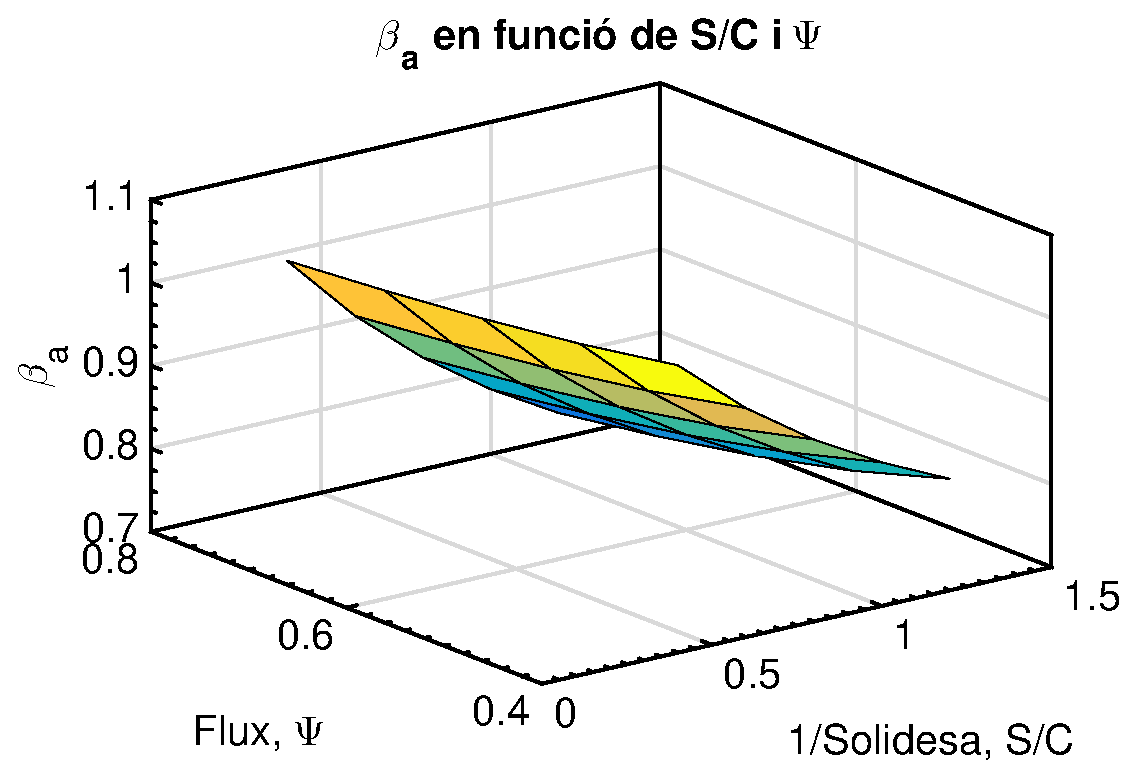
\includegraphics[width=0.8\textwidth]{./code/figures/parametres/betA}
	\caption{Valors de $\beta_a$ en funció de $S/C$ i $\Psi$.}
	\label{betA}
\end{figure}

\begin{figure}[H]
	\centering
	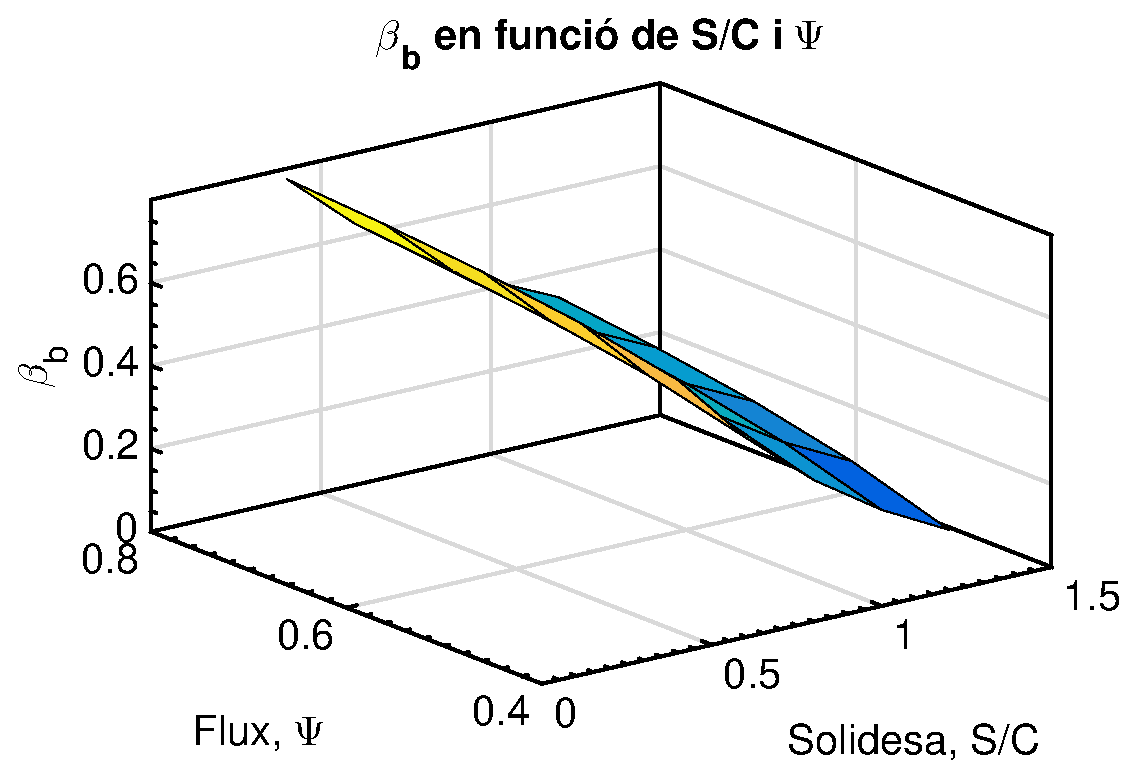
\includegraphics[width=0.8\textwidth]{./code/figures/parametres/betB}
	\caption{Valors de $\beta_b$ en funció de $S/C$ i $\Psi$.}
	\label{betB}
\end{figure}

\subsection{Càlcul de $C_D$ i $C_L$ en funció de $S/C$ i $\Psi$}

\subsection{Càlcul del rendiment de l'escaló en funció de $S/C$ i $\Psi$}

\subsection{Velocitat axial en funció de $S/C$ i $\Psi$}

\subsection{Càlcul de la velocitat tangencial en funció de $S/C$ i $\Psi$}

\subsection{Càlcul del treball de l'escaló en funció de $S/C$ i $\Psi$}

\subsection{Càlcul de la relació de radis en funció de $S/C$ i $\Psi$}

\subsection{Càlcul del radi exterior, radi interior, radi mitjà i altura en funció de $S/C$ i $\Psi$}

\subsection{Càlcul de la velocitat de gir en funció de $S/C$ i $\Psi$}